\chapter{RespVis Packages and Modules}
\label{chap:Packages}

The source code of RespVis is structured into packages containing
modules written in the ES module format. Currently, all packages are
combined into a single, monolithic package during the build process,
but this will be changed in the future so that visualization authors
can import only the packages they need. The reason for this is that
most authors will likely require only a subset of all the features
included in the library, and it would unnecessarily increase the size
of their bundles to import them all. A good example of this is D3,
which also separates its extensive collection of functionality into
different packages, which can be successively added to a project as
the need arises.

At the time of writing, the RespVis library comprises six packages:
the Core package, Legend package, Tooltip package, Bar package, and
Point package, each containing various modules grouped by thematic
similarity. The Core package holds the core functionality of the
library which all other packages depend on. This packages includes the
Layouter and Axis modules, Chart and Chart Window base modules, and
various utility functions and types. The Legend package contains a
Legend module to visualize non-spatial data via labeled symbols. The
Tooltip package holds functions to control the display, placement, and
content of tooltips, as well as utility functions to simplify their
configuration and initialization in Series modules. The Bar package
distinguishes between single-series, grouped, and stacked bars and
includes various low-level and high-level modules to render each of
those types. Similarly, the Line and Point packages contain low-level
and high-level modules to visualize line charts and point charts
(scatterplots), respectively. The different packages and the
dependencies between them are shown in Figure~\ref{fig:Packages}.



\begin{figure}[tp]
\centering
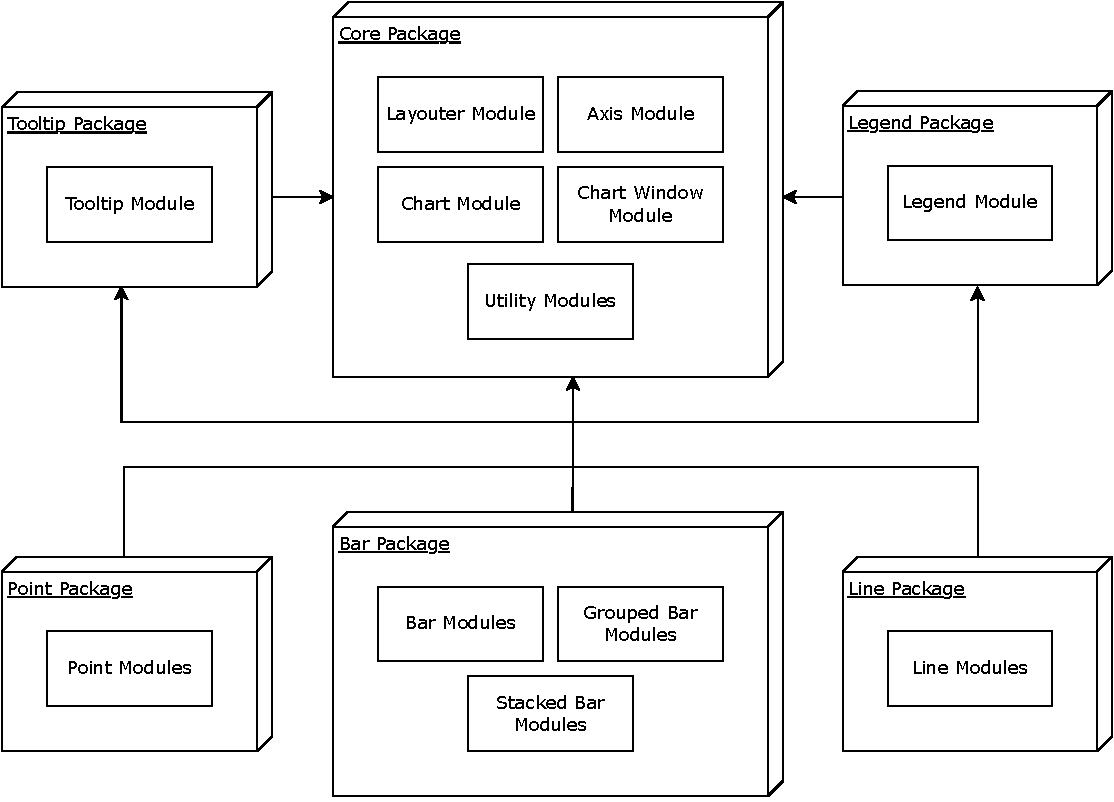
\includegraphics[keepaspectratio,width=\linewidth,height=\fullh]
{diagrams/respvis-packages.pdf}
\caption[Packages of RespVis]{
The six packages of the RespVis library and their most important modules. The
directional arrows indicate dependencies between packages.
\imgcredit{Image created by the author of this thesis using
\href{https://diagrams.net/}{diagrams.net}.}
}
\label{fig:Packages}
\end{figure}







\section{Core Package}

The Core package is located in the \code{src/lib/core/} directory of
the project and contains the necessary core modules of the library. It
forms the base upon which all other packages depend, and includes
various utility functions, the Layouter module, Axis module, Chart
base module, and Chart Window base module. RespVis heavily relies on
utility functions to reuse recurring operations, and the Core package
contains utilities which simplify the handling of arrays, elements, D3
Selections, texts, positions, sizes, rectangles, circles, and paths.
The Layouter module enables the layout of SVG elements with CSS. The
Axis module has been included in the Core package because axes are
important visualization components which occur in nearly all
visualizations. Lastly, the Core package offers Chart and Chart Window
base modules for the creation of more specialized Chart and Chart
Window modules.




\subsection{Utility Modules}

The utilities provided by RespVis are split into multiple modules
placed in the \code{utilities/} directory of the Core
package. These modules include types and functions to perform array,
element, D3 Selection, and text operations, as well as modules to
simplify geometric operations with positions, sizes, rectangles,
circles, and paths. Utility functions are grouped into modules by the
type of entity on which they operate, which is is also reflected in
the utility function names. The names of utility functions follow the
top-down naming convention described in
Section~\ref{sec:NamingConventions}, which means that the names all
begin with the type of entity with which the function is associated.

Array utilities can be found in the Array Utility module in
the \code{utilities/array.ts} file. The \code{Array} class in the
JavaScript base implementation already offers a wide variety of
convenient methods to work with arrays. These methods form a solid
foundation to handle a broad range of situations, but not everything
is covered, and some things require manual implementations, which is
why the RespVis library offers additional functions to simplify
commonly encountered tasks. The \code{arrayEquals} function is used to
verify the equality of two arrays and also works with arbitrary levels
of nesting. Array type guard functions are used to determine at
runtime whether or not a variable is an array. The function
\code{arrayIs} evaluates to \code{true} if the passed parameter is any
kind of array, and \code{arrayIs2D} evaluates to \code{true} if the
passed parameter is a two-dimensional array. The \code{arrayIs}
function is merely an alias for the \code{Array.isArray} method and
has been added to provide a consistent counterpart to the
\code{arrayIs2D} type guard function. The last function in the
Array Utility module is the \code{arrayPartition} function,
which receives an array and a partition size as parameters and returns
a partitioned version of the input array with each chunk containing
the number of items specified by the partition size parameter.


The Element Utility module located at \code{utilities/elements.ts} in
the Core package contains functions and constants related to elements
in a document. The \code{elementRelativeBounds} function is used to
calculate the bounding box of an element relative to the bounding box
of its parent in viewport coordinates. Internally, it uses the
\code{getBoundingClientRect} function, which returns the actual
bounding box of an element in viewport coordinates and, as opposed to
other ways of accessing this information, this function also takes
transformations into account. Every element has a set of CSS styles
applied to them, and the \code{Window.getComputedStyle} method is used
to query the active styles of elements. The style declaration object
returned by this method contains all possible CSS properties and their
values, regardless of whether or not they are set to default values.
Sometimes this behavior may be desired, but in this library, the
computed style is mainly used for the preparation of a downloadable
SVG document to transform styling information set in CSS to attributes
on the individual elements. If every possible CSS property on every
element would be mapped to an attribute, the resulting SVG document
would be unnecessarily bloated and hard-to-read, because only those
properties that are not set to their default values actually have an
effect. For this reason, the
\code{elementComputedStyleWithoutDefaults} function has been
implemented to calculate the computed style of an element and remove
all default-valued properties from the returned style declaration
object. This is implemented by adding a \elname{<style-dummy>} element
as a sibling of the element of interest, computing the styles of both
elements, and calculating the difference between them. To accelerate
these calculations, the \code{elementComputedStyleWithoutDefaults}
function accepts an array of property names as its second parameter
and will only consider the properties listed in this array. The
constant \code{elementSVGPresentationAttrs} array contains the names
of all SVG presentation attributes listed in the SVG 1.1 specification
\parencite{SVG11}. As soon as support for SVG 2 \parencite{SVG2} by
most major browsers has reached maturity, this array will be extended
to include any newly added presentation attributes. Since only these
SVG attributes can be styled via CSS, only CSS properties representing
presentation attributes have to be considered when preparing
downloadable SVG documents.

D3 Selection utilities are implemented in the Selection Utility module
in the \code{utilities/selection.ts} file. They include typing
improvements for the D3 \code{Selection}, \code{Transition}, and
\code{SelectionOrTransition}\ interfaces, and include type guards to
distinguish between them. The D3 \code{Selection}, \code{Transition},
and \code{SelectionOrTransition} interfaces allow the specification of
four type variables: the type of elements contained in the Selection
or Transition, the type of data bound to those elements, the type of
the parents of those elements, and the type of data bound to those
parents. In most cases, the type variables related to parent elements
do not influence the logic of code using these interfaces and could be
omitted to keep it more concise. For this reason, these interfaces
have been re-exported with default types set on all of the type
variables, which means that whenever type variables need to be
manually specified, only those that need to be set to specific types
need to be explicitly stated. Further typing improvements have been
made to the \code{attr} and \code{dispatch} methods of the
\code{Selection} interface. The D3 type declarations of the
\code{Selection.attr} method do not include \code{null} as a possible
return value, which is wrong because this method will result in a
\code{null} value when reading an attribute that does not exist. To
fix this inconsistency and catch potential bugs related to it during
compilation, the type declaration of the \code{Selection.attr} method
has been overwritten in the Selection Utility module to include
\code{null} as a possible return value. A less important but
convenient improvement has been made to the type declaration of the
\code{Selection.dispatch} method, which allows the dispatching of
custom events with certain parameters that control different aspects
of how this event is dispatched and the data bound to it. In practice,
not all parameters need to be specified at every invocation because
the implementation of the \code{Selection.dispatch} method will
provide default values for all of them, but this is not reflected in
the type declaration of the function, which requires every parameter
to be set every time the function is called. To fix this, the
Selection Utility module provides a type declaration overwrite for the
\code{Selection.dispatch} function that wraps the type of the
parameters parameter into the native \code{Partial} utility
type. Apart from these typing improvements, this module also provides
the \code{isSelection} and \code{isTransition} type guard functions
that are used to distiguish between D3 Selections and Transitions.


Utilities for dealing with \elname{<text>} elements can be found in the
Text Utility module in the \code{utilities/text.ts} file, which contains
basic functionality to set specific \attrname{data-*} attributes to
specific values on \elname{<text>} elements. The Text Utility module
holds functions that set \attrname{data-*} attributes controlling the
horizontal and vertical alignment of \elname{<text>} elements, as well
as their orientation. Horizontal and vertical alignment is configured
using the \code{textAlignHorizontal} and \code{textAlignVertical}
functions, which respectively set the \attrname{data-align-h} and
\attrname{data-align-v} attribute on \elname{<text>} elements to the value
passed into either function as a string enum parameter of type
\code{HorizontalAlignment} or \code{VerticalAlignment}. The
\code{HorizontalAlignment} enum represents the string values
\code{\"left\"}, \code{\"center\"} and \code{\"right\"}, while the
\code{VerticalAlignment} enum represents the values \code{\"top\"},
\code{\"center\"} and \code{\"bottom\"}. The distinct
\attrname{data-align-h} and \attrname{data-align-v} attribute values are then
used in selectors of various CSS rules to declare different values for
the CSS \cssname{text-anchor} and \cssname{dominant-baseline} properties. Text
orientation is set using the \code{textOrientation} function, which
sets the \attrname{data-orientation} attribute on \elname{<text>} elements
to the value specified via the \code{Orientation} string enum
parameter. The \code{Orientation} enum represents the values
\code{\"horizontal\"} and \code{\"vertical\"}. These
\attrname{data-orientation} attribute values are then used in CSS to set
the CSS \cssname{text-anchor}, \cssname{dominant-baseline}, and \cssname{transform}
properties of \elname{<text>} elements, in order to rotate them
accordingly and position them correctly inside their bounding box
calculated by the Layouter.


The Core package also contains utilities to simplify geometric
operations. One of these utility modules is the Position Utility
module located in the \code{utilities/position.ts} file, which
contains the \code{Position} interface and various functions to
perform operations related to it.  The \code{Position} interface
consists of the \code{x} and \code{y} number properties. Rounding
these properties is necessary to be able to correctly compare the
equality of two \code{Position} objects and to not render
unnecessarily long strings when transforming them into string
representations. This rounding is performed with the
\code{positionRound} function, which allows the specification of the
number of decimals the properties should be rounded to. Equality
comparision between two \code{Position} objects can be done with the
\code{positionEquals} function, which evaluates to \code{true} if all
properties of both \code{Position} objects are equal and \code{false}
if not. The \code{positionToString} function can be used to transform
a \code{Position} object into its \code{\"x, y\"} string
representation, and its counterpart, the \code{positionFromString}
function, can be used to transform a correctly-formatted string into a
\code{Position} object. A large part of RespVis consists of modifying
the attributes of elements. The \code{positionToAttrs} function can be
used to set the \attrname{x} and \attrname{y} attributes of elements
to the values of the \code{x} and \code{y} members of a
\code{Position} object, and similarly, the
\code{positionToTransformAttr} function can be used to set the
\attrname{transform} attribute of elements to a translation
representing a \code{Position} object. The Position Utility module
also contains the \code{positionFromAttrs} function, which can be used
to create a \code{Position} object from an element's \attrname{x} and
\attrname{y} attributes.

The Size Utility module located in the
\code{utilities/size.ts} file in the Core package is very
similar to the Position Utility module. It contains the
\code{Size} interface, which consists of the \code{width} and
\code{height} number properties, the \code{sizeRound} function to
round the properties of a \code{Size} object to a certain number of
decimals, and the \code{sizeEquals} function to compare two
\code{Size} objects for equality. Similar to the equivalent functions
in the Position Utility module, the \code{sizeToString} and
\code{sizeFromString} functions can be used to convert between
\code{Size} objects and their string representations, and the
\code{sizeToAttrs} and \code{sizeFromAttrs} functions can be used to
convert between \code{Size} objects and \attrname{width} and
\attrname{height} attributes of elements.

Utilities for dealing with rectangles can be found in the
Rectangle Utility module, which is located in the
\code{utilities/rect.ts} file of the Core package. This
module contains the \code{Rect} interface, which is the union of the
\code{Position} and \code{Size} interfaces and therefore describes an
object with the \code{x}, \code{y}, \code{width}, and \code{height}
number properties. Similar to the Position and Size Utility Modules,
this module contains the \code{rectRound} function to round
\code{Rect} objects, the \code{rectEquals} function to compare two of
them for equality, the \code{rectToString} and \code{rectFromString}
functions to convert between \code{Rect} objects and their string
representations, and the \code{rectToAttrs} and \code{rectFromAttrs}
functions to convert between objects and \attrname{x}, \attrname{y},
\attrname{width}, and \attrname{height} attributes of elements. Since
the \code{Rect} interface is a combination of the \code{Position} and
\code{Size} interfaces, most of the functions in this module
internally use the functions provided by the Position and
Size Utility modules. The \code{rectMinimized} function
creates a minimized version of the passed \code{Rect} object, which is
infinitely small and positioned at the original \code{Rect} object's
center. Minimized rectangles are used in transitions that grow or
shrink \elname{<rect>} elements from or to their centers. When
declaring a stroke for SVG elements, it is drawn exactly on the
outline of an element's shape, which means that a stroke will extend
outside the original bounds of an element by half the stroke width.
This can lead to unwanted artifacts like the stroke of bars in a bar
chart overlapping over the chart's axes. To counteract this, the
\code{rectFitStroke} function is offered by the Rectangle
Utility module to adjust the properties of \code{Rect} objects to
account for a specific stroke width around them. Lastly, the
Rectangle Utility module provides functions to calculate
specific positions inside rectangles. The most generic of these
functions is the \code{rectPosition} function, which enables the
calculation of a position inside a rectangle via a two-dimensional
parameter that expresses a position as the percentual width and height
distance from a rectangle's top-left corner. All other
position-calculating rectangle utility functions are simply shorthand
functions that internally call the \code{rectPosition} function. The
\code{rectCenter} function returns a \code{Position} object
representing the center position of a \code{Rect} object. The
\code{rectLeft}, \code{rectRight}, \code{rectTop}, and
\code{rectBottom} functions return \code{Position} objects that
represent the middle position of the corresponding edge of a
\code{Rect} object. Similarly, The \code{rectTopLeft},
\code{rectTopRight}, \code{rectBottomRight}, \code{rectBottomLeft}
functions can be used to calculate the corner positions of a
rectangle.

The Circle Utility module can be found in the
\code{utilities/circle.ts} file in the Core package. It
contains the \code{Circle} interface, which describes a circle via a
\code{center} \code{Position} property and a \code{radius} number
property. This module also contains equivalent functions to those
found in previously-mentioned utility modules: \code{circleRound},
\code{circleEquals}, \code{circleToString}, \code{circleFromString},
\code{circleToAttrs}, \code{circleFromAttrs}, \code{circleMinimized},
and \code{circleFitStroke}. Furthermore, the \code{circlePosition}
function can be used to calculate positions inside a circle using an
angle that defines an offset direction and an offset distance from a
circle's center as a percentage of the circle's radius. The
Circle Utility module also contains functions to create
circles from rectangles, which are the \code{circleInsideRect}
function to calculate the largest circle that can fit inside of a
rectangle and the \code{circleOutsideRect} function to calculate the
smallest circle that encloses a rectangle.

The Path Utility module is located in the \code{utilities/path.ts}
file in the Core package and provides functions to simplify the
creation of path definitions that can be set as \attrname{d} attributes on
\elname{<path>} elements. The \code{pathRect} function uses a
\code{Rect} object to create a rectangle path definition that can be
set on \elname{<path>} elements instead of using \elname{<rect>} elements.
Similarly, the \code{pathCircle} function uses a \code{Circle} element
to create a circle path definition that can be set on \elname{<path>}
elements instead of using a \elname{<circle>} elements. The reasons for
using \elname{<path>} elements rather than more descriptive shape
elements is that their shapes can be changed dynamically and it
is possible to smoothly transition between shapes by interpolating
their path definition strings.





\subsection{Layouter Module}
\label{sec:Layouter}

The Layouter module is the most significant contribution of this
work. A Layouter wraps around an SVG document and allows configuration
of the layout of elements in this document with CSS mechanisms like
Grid and Flexbox. Instead of implementing a custom layout algorithm,
the Layouter utilises the layout engines already built into browsers,
which were summarized in Section~\ref{sec:BrowserEngines}. Earlier
proof of concept implementations used the FaberJS \parencite{FaberJS}
and Yoga \parencite{Yoga} layout engines to compute layouts, but these
implementations limited layouting to either Grid-based or
Flexbox-based constraints. The use of built-in browser functionality
in the current implementation leads to visualization authors being
able to use all the layouting capabilities natively offered by
browsers, as well as reduced bundle sizes.

CSS has always been the foundation of responsive web design for
HTML-based websites, because of its ability to adapt an element's
presentation and the possibility of defining different presentations
for different contexts via media queries. A large part of the
responsive power of CSS comes from its ability to change the
positioning and layout of elements. As already mentioned in previous
chapters, CSS can style certain aspects of SVG documents, but it is
not possible to use CSS layouting mechanisms to position SVG elements.
Although other visualization libraries such as Chartist
\parencite{Chartist} and Highcharts \parencite{Highcharts} allow the
use of CSS to style visualizations, none of them offer the possibility
to modify the layout of visualizations via CSS. Instead, visualization
authors have to learn and use custom APIs to position elements,
limiting the range of possible layouts to those supported by the
individual libraries.

The RespVis Layouter module distinguishes between laid-out and
non-laid-out elements, since not every element in a visualization
profits from being laid out. The positions and sizes of laid-out
elements are calculated by the Layouter, whereas non-laid-out elements
are ignored during the layout process.  Theoretically, the Layouter
could be used to position all visualization elements, since all that
is necessary is to determine a good mapping for each element that maps
the rectangular bounding box calculated by the Layouter to the desired
SVG shape of the element. However, the positioning of elements in a
visualization is constrained more strictly than element positioning in
typical HTML documents, since the content of a visualization is
communicated through visual features such as position, size, shape,
and poximity of elements, rather than simply through text which can be
positioned much more freely. For this reason, many elements of a
visualization must be positioned at specific locations with specific
dimensions, which means there is very little profit in laying them out
with an elaborate layout algorithm. Hence, exactly-positioned elements
like the \elname{<rect>} elements of Bar Series and the
\elname{<circle>} elements of Point Series are usually positioned
directly via their SVG attributes.


Using the Layouter requires a more complex rendering process than
would be needed if the boundaries of elements would already be known
before rendering them. The way the Layouter works, elements affecting
the layout need to be pre-rendered in advance, and afterwards, when
the positions and sizes of elements are known, the visualization needs
to be rerendered in its final form. This leads to the three-phased
rendering process shown in Figure~\ref{fig:RenderProcess}. The three
phases are: 1.\ the First Render phase to render elements affecting
the layout, 2.\ the Layout Process, and 3.\ the Second Render phase to
render elements affected by the layout. The elements affecting the
layout of the visualization are mainly laid-out container
\elname{<svg>} and \elname{<g>} elements containing exactly-positioned
child elements. Dynamically-sized elements such as \elname{<text>}
elements and axes also need to be fully rendered in the First Render
phase. The Layout Process is where the Layouter calculates the layout
of a visualization using the process described in the following
paragraphs. In the Second Render phase, the bounding boxes calculated
during the Layout Process are used to perform a second rendering of
the complete visualization. Here, every element affected by the
layout, i.e. nearly every element, is rendered at its final position
with its final dimensions. In theory, the two render phases could be
implemented as separate functions, but it is more convenient to just
invoke the same render function twice and perform some operations only
if the boundaries of elements have already been calculated.


\begin{figure}[tp]
\centering
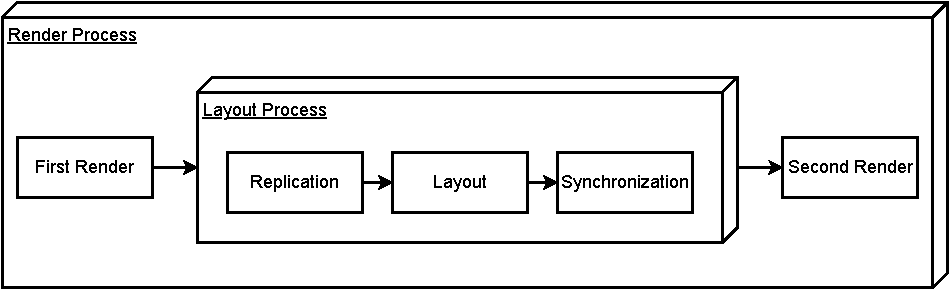
\includegraphics[keepaspectratio,width=\linewidth,height=\thirdh]
{diagrams/respvis-render-process.pdf}
\caption[Render Process When Using the Layouter]{%
The three phases of the RespVis Layouter's Render Process:
First Render, Layout Process, and Second Render.
During the First Render phase, every element which affects
the layout needs to be rendered. The second phase consists of the
Layout Process performed by the Layouter. The Layout Process includes
three steps: a) Replication, in which laid-out SVG elements are replicated with
\elname{<div>} elements, b) Layout, in which these \elname{<div>}
elements are automatically laid out by the browser, and
c) Synchronization, in which the bounding boxes of the laid out
\elname{<div>} elements are set as \attrname{bounds} attributes on the
original SVG elements. In the Second Render phase, the calculated
boundaries are used to re-render all elements of the visualization in
their final positions with their final dimensions.
\imgcredit{Image created by the author of this
thesis using \href{https://diagrams.net/}{diagrams.net}.}
}
\label{fig:RenderProcess}
\end{figure}


The Layouter Module can be found in the \code{layouter.ts} file of the
Core package. The main function of this module is the
\code{layouterCompute} function which implements the three-stepped
Layout Process shown in the middle of
Figure~\ref{fig:RenderProcess}. The three steps are:
\begin{enumerate}
\item[a)] Replication: The structure of the SVG document to be laid
  out is replicated with HTML \elname{<div>} elements, because only
  HTML elements can be affected by CSS-based positioning. These
  elements are referred to as \enquote{layout elements} and have the
  same classes and \attrname{data-*} attributes as the SVG elements
  they are replicating.

\item[b)] Layout: The replicated layout elements are affected by CSS
  rules to configure their positioning and are automatically laid out
  by browsers. If the selectors of CSS rules used to style SVG
  elements only select them using classes and \attrname{data-*}
  attributes, the layout of these elements can be directly configured
  in these rules, since the corresponding layout elements have the
  same classes and \attrname{data-*} attributes.

\item[c)] Synchronization: In this step, the positions of layout
  elements are synchronized with their respective SVG elements. The
  calculated bounding boxes of layout elements are set as
  \attrname{bounds} attributes on SVG elements to make the boundary
  information available in subsequent renderings for the positioning
  of nested elements. In addition, the Layouter sets different default
  attributes on different types of SVG elements that aim to represent
  the boundaries of individual elements.
\end{enumerate}


During the replication process, the structure of an SVG document is
replicated with HTML \elname{<div>} elements, which is implemented via
a hierarchical D3 data join, in which the original SVG elements are
bound as data objects to layout elements. The hierarchical data join
results in a counterpart in the hierarchy of layout elements for each
SVG element that should be affected by the Layouter. Since
not every SVG element should be positioned via the Layouter,
the Layouter must be told which elements to ignore. For
this, the \attrname{data-ignore-layout} and
\attrname{data-ignore-layout-children} attributes have been
introduced. Elements having the \attrname{data-ignore-layout}
attribute or which are children of elements having the
\attrname{data-ignore-layout-children} attribute will not be
replicated and laid out by the Layouter.

To configure the layout of such layout elements in CSS, it must be
possible to select them uniquely with a CSS selector. This selector
should be as similar as possible to the selector of their
corresponding SVG elements, to make it as easy as possible to
configure the CSS properties of layout elements. For this purpose, the
\code{class} attributes and all \attrname{data-*} attributes of SVG
elements are copied to their layout elements. In addition to the
classes of the replicated SVG element, the \code{layout} class is set
on all layout elements, which makes it possible to specifically select
an SVG element's layout element via the same selector extended by the
\code{layout} class. If CSS rules affecting SVG elements use only
classes and \attrname{data-*} attributes in their selectors, the
properties of corresponding layout elements can be directly configured
in the same rules, since these selectors will also match them. An
example of how an SVG document is replicated with \elname{<div>}
layout elements can be seen in Figure~\ref{fig:LayouterReplication}.

\begin{figure}[tp]
\centering
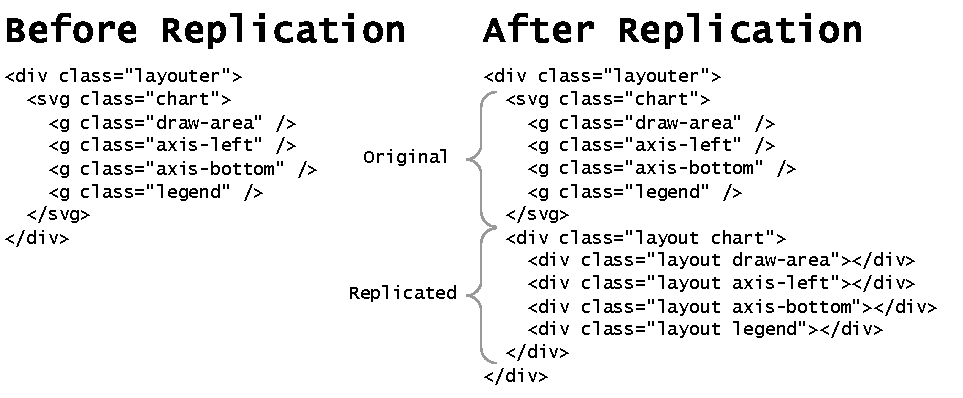
\includegraphics[keepaspectratio,width=\linewidth,height=\thirdh]
{diagrams/respvis-layouter-replication.pdf}
\caption[Replication of an SVG Document via Layouter]{%
The replicated layout element structure of an SVG document. Every SVG
element has a corresponding layout element with the same classes
and \attrname{data-*} attributes. In addition to the classes of the
original SVG element, every layout element also has the \code{layout}
class to allow specific targeting of layout elements via CSS
selectors.
\imgcredit{Image created by the author of this thesis using
\href{https://diagrams.net/}{diagrams.net}.}
}
\label{fig:LayouterReplication}
\end{figure}


The size of dynamically-sized elements depends on the size of their
content. Since layout elements exist separately from their SVG
elements and cannot access their content, a manual solution had to be
implemented to set the size of layout elements to the content size of
their SVG elements when required. \elname{<text>} elements are a good
example of dynamically-sized elements, because their size is rarely
explicitly declared and usually depends on the size of their textual
content. The custom CSS \cssname{--fit-width} and
\cssname{--fit-height} properties were introduced to activate the
manual copying of dimensions from SVG elements to their layout
elements. These boolean properties can be set in CSS rules and are
checked during the Replication step via the
\code{window.getComputedStyle} method. If at least one of these
properties is set to \code{true}, the dimensions of the SVG element
are calculated with the \code{Element.getBoundingClientRect} method
and are set as \cssname{width} or \cssname{height} properties in the
\attrname{style} attribute on the corresponding layout element. This
way, layout elements will have the same sizes as their SVG elements
and can be properly used in the calculation of the overall layout.

Layout elements are positioned according to the layout information
specified in CSS rules during the Layout step. Since layout elements
are merely \elname{<div>} elements which have been styled via CSS rules,
the browser can position them automatically via its integrated layout
engine, which happens immediately after they have been created or
updated in the Replication step. After the Layout step, the final
bounding boxes of layout elements can be calculated and used for
further operations.

In the Synchronization step of the Layout Process, the Layouter
calculates the bounding boxes of all layout elements and sets this
boundary information as attributes on the corresponding SVG
elements. Bounding boxes of layout elements are calculated relative to
their parent elements using the \code{elementRelativeBounds} utility
function, converted to their string representations via the
\code{rectToString} utility function, and set as \attrname{bounds}
attributes on corresponding SVG elements.  These \attrname{bounds}
attributes can then be deserialized to \code{Rect} objects whenever
the bounding boxes of SVG elements are needed for calculations in
subsequent renderings. In addition to setting \attrname{bounds}
attributes, the Layouter also sets specific default attributes on
different types of SVG elements in an attempt to automatically fit
them into their bounding boxes without manually having to set
attributes in subsequent renderings. If the Layouter would not set
these default attributes, they would have to be set manually on every
laid-out element in the rendering functions, which would be less
convenient and lead to duplicated code in various places. For those
SVG elements which can be mapped directly to rectangular areas, such
as \elname{<svg>} and \elname{<rect>} elements, the \attrname{x},
\attrname{y}, \attrname{width}, and \attrname{height} attributes are
set to the values of the element's bounding boxes. SVG shape elements
which have explicit sizes and positions but are not rectangular, such
as \elname{<circle>} and \elname{<line>} elements, also receive
attributes that fit them into their boundaries in a way that was
deemed most sensible. Other SVG elements which are not explicitly
sized, such as \elname{<g>} and \elname{<text>} elements, are merely
moved to the correct positions by setting their \attrname{transform}
attributes to translations so that their top-left corners align with
the top-left corners of their bounding boxes. The Layouter does not
automatically reposition exactly-positioned elements based on the
changed boundary of the composite \elname{<svg>} or \elname{<g>}
elements containing them, so this has to be implemented manually in
the render functions of various components.









\subsection{Axis Module}

Axes are implemented in the \code{axis.ts} Axis module in the Core
package and are used to visualize scales that map abstract values to
spatial dimensions. Currently, only Cartesian axes, distinguished by
their position relative to a visualization's draw area, are provided
by RespVis, since only Cartesian Charts have been implemented so
far. Furthermore, the implementation has so far been focused on Left
and Bottom axes, because they are the most commonly encountered types
of Cartesian axes and cover most use cases. An Axis consists of ticks,
an optional title, and an optional subtitle, where the ticks are the
actual visualization of a spatial-mapping scale, and the title and
subtitle can be specified for additional description. An example of
what a rendered Left and Bottom Axis might look like can be seen in
Figure~\ref{fig:Axes}.

\begin{figure}[tp]
\centering
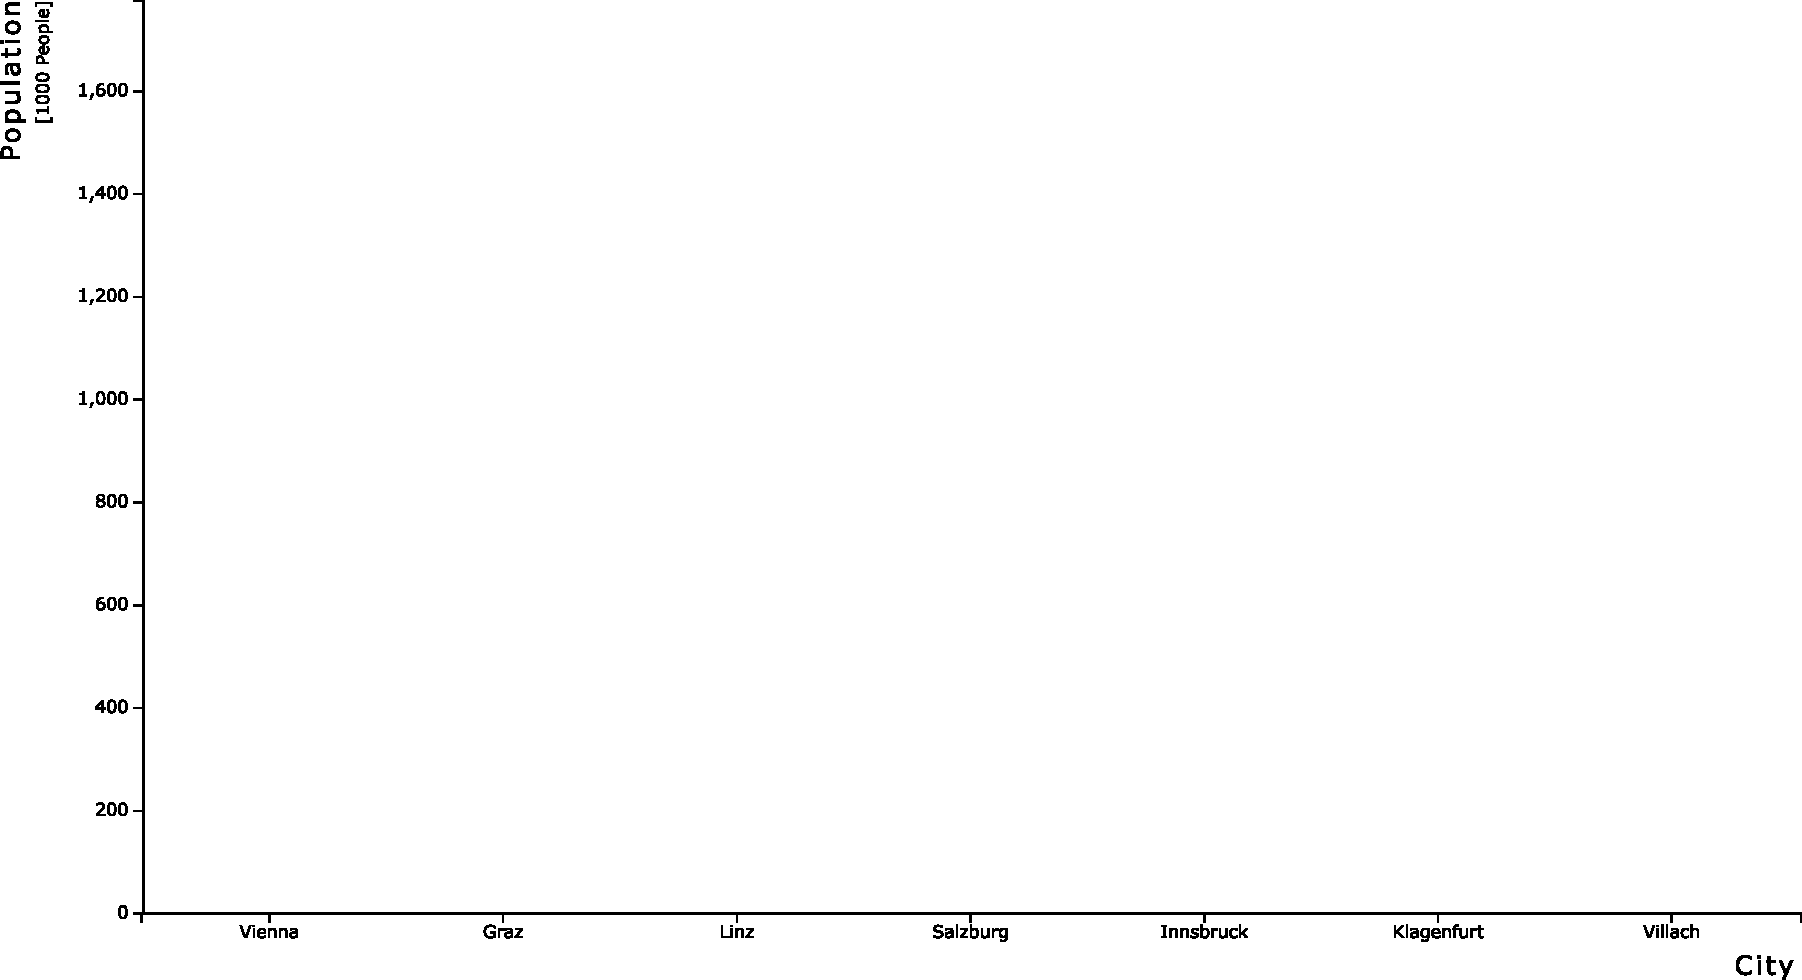
\includegraphics[keepaspectratio,width=\linewidth,height=\halfh]
{diagrams/axes.pdf}
\caption[Axes Example]{%
A rendered Left Axis with ticks, a title, and a subtitle, and a
Bottom Axis with ticks and a title.
\imgcredit{Image created by the author of this thesis using RespVis
  and \href{https://inkscape.org/}{Inkscape}.}
}
\label{fig:Axes}
\end{figure}


The \code{Axis} interface describes the shape of a data object with
which an Axis can be configured. It includes a \code{scale} property,
representing the scale to be visualized, the \code{title} and
\code{subtitle} string properties, and the \code{configureAxis}
function property, which can be used to configure the underlying D3
Axis before rendering it. Like most other modules, the Axis module
consists of two main functions: a data creation function and a render
function. The \code{axisData} function is used to create an
\code{Axis} data object from a \code{Partial<Axis>} object parameter,
where all non-set but required properties are filled with default
values. The \code{axisBottomRender} and \code{axisLeftRender}
functions are used to render a Left and Bottom Axis in a composite
element on which an \code{Axis} data object has been bound. An Axis'
root element is a CSS Grid container and defines the layout of the
title, subtitle, and ticks elements. The default configuration of a
Left Axis positions these elements in a three-column layout in which
the title, subtitle, and ticks elements are placed in this order from
left to right. For a Bottom Axis, the default configuration positions
the same elements in a three-row layout, in which the ticks, title,
and subtitle elements are placed in this order from top to bottom.
Furthermore, the title and subtitle elements of a Left Axis are
oriented vertically to save horizontal space using the
\code{textOrientation} utility function. Internally, the Axis module
uses the \code{axisBottom} and \code{axisLeft} functions from the D3
Axis package \parencite{D3Axis} to render the ticks of an Axis. Since
these D3 functions use attributes to position and style elements, as
many of these attributes as possible must be removed directly after
the ticks have been rendered to enable their configuration via CSS.






\subsection{Chart Module}
\label{sec:Chart}

Charts are high-level components which represent a complete
visualization with Axes, Legends, and Series. An example of a rendered
RespVis Chart containing a Left Axis, a Bottom Axis, a Grouped Bar
Series, a Label Series, and a Legend can be seen in
Figure~\ref{fig:Chart}. A Chart is typically rendered into the root
\elname{<svg>} element of an SVG document. The \code{chartRender}
function from the \code{chart.ts} Chart module in the Core
package can be used to set the necessary classes and attributes on
these \elname{<svg>} elements.


\begin{figure}[tp]
\centering
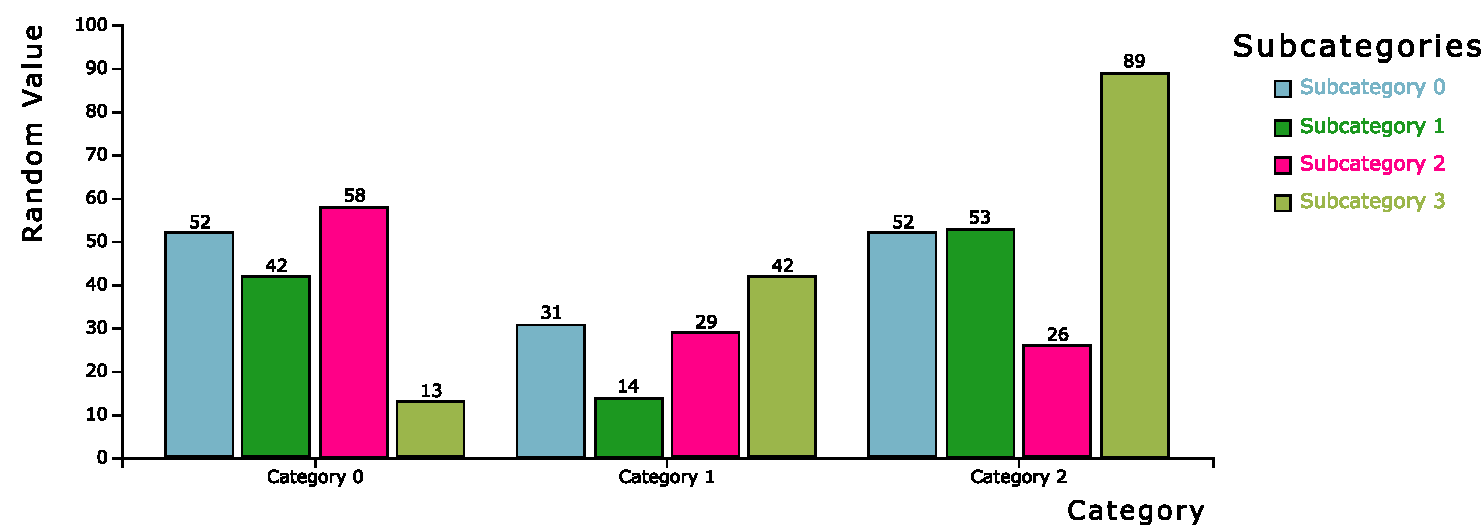
\includegraphics[keepaspectratio,width=\linewidth,height=\fullh]
{diagrams/chart.pdf}
\caption[Cartesian Chart Example]{%
A Cartesian Chart containing a Left Axis, a Bottom Axis,
a Grouped Bar Series, a Label Series, and a Legend.
\imgcredit{Image created by the author of this thesis.}
}
\label{fig:Chart}
\end{figure}


As mentioned previously, RespVis currently only supports Cartesian
Charts, which visualize data in a Cartesian coordinate system. The
Cartesian Chart base module is located in the
\code{chart-cartesian.ts} file in the Core package. The
\code{ChartCartesian} interface describes a data object for the
configuration of Cartesian Charts via the \code{xAxis} and
\code{yAxis} \code{Axis} properties which describe the x and y Axes of
the Chart respectively. Transposing Axes is a useful pattern to
improve the responsiveness of visualizations and can be configured
using the \code{flipped} boolean property of a Cartesian Chart's data
object. If the \code{flipped} property is set to \code{false}, the
\code{xAxis} object is used to configure the Bottom Axis and the
\code{yAxis} object is used to configure the Left Axis. If it is set
to \code{true}, it is the other way around.

The \code{chartCartesianData} function is used to create a
Cartesian Chart's data object. This function gets a partial data
object with only those properties set which are of interest to the
calling code, and all non-set properties are filled with default
values. The default values of the \code{xAxis} and \code{yAxis}
properties are set by the \code{axisData} function from the Axis
module. The \code{flipped} property is initialized to \code{false}.

The rendering of Cartesian Charts is split into two functions, which
have to be called separately, because not all parts of a Cartesian
Chart can be rendered simultaneously. The general structure of a Chart
must be rendered before anything else can be rendered, since this
includes the draw area container element into which individual Series
are rendered. A Chart's Axes need fully initialized scales to be
rendered correctly. However, the range of a scale, i.e. the range of
values into which abstract values are mapped, depends on the size of
the draw area and is only set during the render function of the
individual Series. Therefore, a Cartesian Chart's Axes must be
rendered after its Series in order to ensure fully initialized scales.

The structure of a Cartesian Chart is rendered with the
\code{chartCartesianRender} function, which sets the necessary
attributes and classes on the root element and attaches the draw area
\elname{<svg>} element to it. The draw area is the container element
into which the Series of a Chart are rendered. An \elname{<svg>}
element without actual content is not able to receive input events,
which means that it would, for example, not be possible to capture
scroll events to control a zoom interaction when the cursor is over
the empty area of the draw area. To counter this, a transparent
\elname{<rect>} background element filling the whole draw area is
added, allowing input events to be received even in empty areas.

The \code{chartCartesianAxesRender} function is used to render the
Axes of a Cartesian Chart. This function must only be called on
elements with a bound \code{ChartCartesian} data object and only after
the scales that are to be visualized by the Axes have been fully
initialized. Charts must first render the Chart's structure using the
\code{chartCartesianRender} function, followed by the desired Series,
and only then can the Chart's Axes be rendered using the
\code{chartCartesianAxesRender} function. The
\code{chartCartesianAxesRender} function creates two \elname{<g>}
elements and renders a Left Axis and a Bottom Axis in them. Depending
on whether the \code{flipped} property in the bound data object is set
to \code{true} or \code{false}, the \code{xAxis} data object is used
to configure the Bottom Axis or Left Axis and the \code{yAxis} data
object is used to configure the other. 

The elements of a Cartesian Chart are positioned using a CSS Grid
layout. By default, a grid is created which defines the
\code{axis-left}, \code{axis-bottom}, \code{draw-area}, and
\code{legend} areas. Most rows and columns of this grid are sized to
fit their content, with the only exception being the row and column
containing the draw area, which are set to fill the remaining space
not occupied by other rows and columns. The default CSS configuration
of a Cartesian Chart positions a potential Legend to the right of the
draw area, but this can be changed by either adjusting the grid
directly via CSS or activating one of the preconfigured positions via
the \attrname{data-legend-position} attribute. To simplify setting the
\attrname{data-legend-position} attribute, the
\code{chartLegendPosition} function can be used, which sets this
attribute to the value of the passed \code{LegendPosition} enum
parameter.






\subsection{Chart Window Module}

The Chart Window module is implemented in the \code{chart-window.ts}
file in the Core package. Chart Windows render a wrapped
Chart inside a Layouter and decorate it with a Toolbar. They
represent an even higher-level layer of abstraction than Charts and
are used to manage their rendering process and configuration. In most
other visualization libraries, Charts are provided as the highest
level of components that can be configured, which typically means that
additional HTML elements for the runtime configuration of Charts have
to be created and managed by the embedding web page itself. Chart
Windows are rendered with the \code{chartWindowRender} function on
HTML \elname{<div>} elements. Their structure consists of a
\elname{<div>} element in which the Toolbar is rendered, and of
another \elname{<div>} element on which a Layouter is
initialized and which holds the wrapped Chart's SVG document. An
example of a Chart Window with an expanded Tool Menu containing two
Nominal Filtering Tools and an SVG Download Tool can be seen in
Figure~\ref{fig:ChartWindow}.


\begin{figure}[tp]
\centering
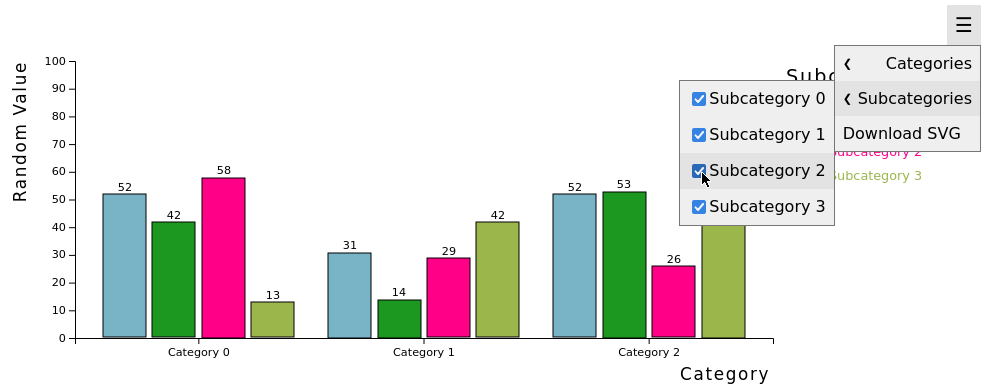
\includegraphics[keepaspectratio,width=\linewidth,height=\fullh]
{images/chart-window.png}
\caption[Chart Window Example]{%
A Chart wrapped in a Chart Window. The Tool
Menu has been expanded by hovering over it, and the menu entries of
two Nominal Filtering Tools and the SVG Download Tool can be seen
inside. \imgcredit{Image created by the author of this thesis.}
}
\label{fig:ChartWindow}
\end{figure}


Currently, the Toolbar only contains the Tool Menu, a dropdown menu
into which individual tools are added as menu items or as submenus.
Dropdown menus are created with the \code{menuDropdownRender} function
and consist of a title and a container for menu items. The current
dropdown menu implementation uses no JavaScript and simply shows menu
items via CSS when there is a hover interaction. The Tool Menu is
created with the \code{menuToolsRender} function, which internally
uses the \code{menuDropdownRender} function to initialize it as a
dropdown menu.

The Core package provides various tools which can be added to the Tool
Menu of Chart Windows. One of these tools is the Nominal Filtering
Tool located in the \code{tools/tool-filter-nominal.ts} file of the
Core package. This tool is used to filter a nominal (or categorical)
data dimension of a visualized dataset via a dropdown menu that
includes a Checkbox Series. Nominal data, in contrast to ordinal or
quantitative data, consists only of labels that do not have a
quantitative value assigned to them and therefore have no inherent
ordering. The data object for the configuration of a Nominal Filter
Tool is described by the \code{ToolFilterNominal} interface, which
contains properties to specify the title of the dropdown menu, the
individual options to be filtered, and the keys of these options. The
\code{toolFilterNominalData} function is used to create a data object
of type \code{ToolFilterNominal} from a partial input object where
undefined properties are being filled with default values. Nominal
Filtering Tools can then be rendered on elements with bound
\code{ToolFilterNominal} data objects using the
\code{toolFilterNominalRender} function, which internally uses the
\code{menuDropdownRender} function to initialize a dropdown menu into
which the checkboxes representing the individual options of the filter
are rendered as menu items.

Checkbox Series are implemented in the \code{series-checkbox.ts} file
in the Core package and render a series of checkboxes consisting of
checkbox \elname{<input>} elements with associated \elname{<label>}
elements. They are configured using data objects in the form of the
\code{SeriesCheckbox} interface, which contains properties to
determine the type of checkbox container elements and the labels of
checkboxes. A data object of this type can be created with the
\code{seriesCheckboxData} function, which creates a complete object
from a partial one. Checkbox Series are rendered using the
\code{seriesCheckboxRender} function, which generates individual
checkboxes using a data join requiring an array of \code{Checkbox}
data objects so that a single data object can be bound to each
checkbox. Individual \code{Checkbox} data objects contain all the data
needed to render a single checkbox and are created by transforming the
\code{SeriesCheckbox} data objects bound on the Series' root element.
Single checkboxes consist of a container element, an \elname{<input>}
checkbox element, and a \elname{<label>} element. In order to
semantically assign the \elname{<label>} elements to their
\elname{<input>} elements, the \attrname{for} attributes on \elname{<label>}
elements must be set to the ids of their corresponding \elname{<input>}
elements. This requires assigning unique ids to \elname{<input>}
elements, which are generated via the \code{uuid} function and set as
\attrname{id} attributes on the \elname{<input>} elements and as \code{for}
attributes on \elname{<label>} elements when the checkbox is first
created. The \code{uuid} function is an alias for the \code{v4}
function from the \code{uuid} npm package \parencite{UUIDPackage} and
is used to generate UUIDs (Universally Unique IDentifiers)
\parencite{UUIDRFC} of the fourth version, which are very likely to be
unique and therefore can be safely used as values for \code{id}
attributes.

The SVG Download Tool is implemented in the
\code{tools/tool-download-svg.ts} file of the Core package and is
included by default in every Chart Window. SVG documents embedded in
HTML documents cannot be downloaded by web consumers as easily as
raster images, which can simply be downloaded with native browser
tools. Instead, SVG documents must be encoded in \code{Blob} objects
and then set as as object URLs in the \code{href} attributes of
\elname{<a>} elements. However, since the presentation of RespVis
visualizations is mainly configured using CSS, the active CSS
properties must first be converted to attributes before the SVG
document can be downloaded. For this, a clone of the whole SVG
document is made to set attributes on the cloned elements without
affecting the rendered visualization. After the document has been
cloned, attributes reflecting the active CSS configuration of the
original elements are set on cloned elements. The active CSS
configuration of the original elements is calculated using the
\code{elementComputedStyleWithoutDefaults} utility function, which
yields a list of CSS properties and their values, only containing
properties that are not set to defaults. After setting all the
necessary attributes on cloned elements, the string representation of
the cloned document is calculated using the \code{Element.innerHTML}
property and encoded in a \code{Blob} object with the content type
\code{image/svg+xml}. At present, the string representation of the SVG
document is not processed further or prettily formatted, which results
in a rather difficult-to-read file and which will be improved in
future work. The \code{Blob} object containing the SVG document is
further transformed into an object URL via the
\code{URL.createObjectURL} method and set in the \attrname{href} attribute
of a newly created \elname{<a>} element. This newly created
\elname{<a>} element is then briefly attached to the \elname{<body>}
element of the active HTML document and clicked using the
\code{Element.click} method, which initiates the download of the final
prepared SVG document. Download SVG Tools can be rendered as menu
items in a Chart Window's Tool Menu with the
\code{toolDownloadSVGRender} function, which initializes them and
triggers the download of the SVG document embedded in the Chart Window
when a visualization consumer clicks on the menu item.





\section{Legend Package}

The Legend package in the \code{src/lib/legend/} directory currently
comprises a single file \code{legend.ts}, containing the implementation
of the Legend module. Legends are used to visualize scales whose
abstract values are not mapped to spatial dimensions in a coordinate
system, but to other visual properties such as colors, shapes, or
sizes. The Legend implemented in this module illustrates such scales
by creating labeled, configurable symbols for every mapping and,
therefore, this component is best suited for the visualization of
discrete value mappings. Continuous data dimensions can still be
visualized with this component, but they must be approximated by
dividing the continuous domain of values into equal discrete steps.
An example demonstrating the use of the Legend package can be found in
the \code{legend.html} file in the \code{src/examples/} folder. An
excerpt from this example can be seen in Listing~\ref{list:Legend},
with its rendering shown in Figure~\ref{fig:Legend}.

\begin{samepage}
\lstinputlisting[%
  float=tp,
  aboveskip=\floatsep,
  belowskip=\floatsep,
  xleftmargin=0cm,              % no extra margins for floats
  xrightmargin=0cm,             % no extra margins for floats
  %
  basicstyle=\footnotesize\ttfamily,
  frame=shadowbox,
  numbers=left,
  label=list:Legend,
  caption={[Code of Legend Example]%
An excerpt from the source code of the example implemented in the
\code{legend.html} file in the \code{src/examples/} directory. When
executed, this code results in the three Legends shown in
Figure~\ref{fig:Legend}. Non-essential parts of the source code have
been removed to focus on Legend-related configurations. The horizontal
Legend is configured with the same data object as the rectangle symbol
Legend, but the items of the horizontal Legend are laid out
horizontally via the CSS \cssname{flex-direction} property.
},
]{listings/legend.html}
\end{samepage}



\begin{figure}[tp]
\centering
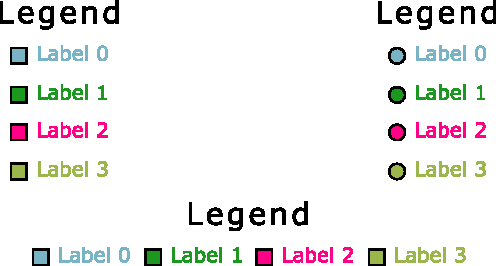
\includegraphics[keepaspectratio,width=\linewidth / 2,height=\fullh]
{diagrams/legend.pdf}
\caption[Legend Example]{%
The three Legends resulting from the source code in
Listing~\ref{list:Legend}. The first Legend has been configured to have
rectangles as symbols, the second to have circles as
symbols, and the third with rectangle symbols horizontally laid out.
\imgcredit{Image created by the author of this thesis.}
}
\label{fig:Legend}
\end{figure}



A data object for the configuration of a Legend is defined by the
\code{Legend} interface, which contains properties to describe the
title, labels, and symbols of a Legend. Symbols are configured via
functions which take the boundaries calculated by the
Layouter into account to set the \attrname{d} attributes of
\elname{<path>} elements. Legend symbols are rendered as
\elname{<path>} elements because these enable the rendering of
arbitrary symbols that can be changed dynamically, whereas the usage
of \elname{<rect>} or \elname{<circle>} elements would be much more
restrictive. A disadvantage of using \elname{<path>} elements is that,
since they require manual configuration of exact shapes via path
definition strings, their usage is more tedious than the usage of more
restricted SVG elements, and they require slightly more annotation
effort when it comes to accessibility. Colors of individual items in a
Legend are indirectly configured via \attrname{data-style} attributes
on items whose values are specified in the \code{Legend} data objects.
Some style classes, such as the \code{categorical-x} classes for
categorical styling, are already provided by RespVis and handled in
the library's distributable CSS file. Furthermore, custom style
classes can easily be added by simply handling them in custom CSS
rules. Legend data objects can be created with the \code{legendData}
function, which receives a partial input object in which the
properties which are not of interest to the calling code are not
required to be set and are populated with default values.

A Legend is rendered into elements which have a Legend data object
bound on them using the \code{legendRender} function. This function
attaches a \elname{<text>} element with which the title of the Legend
is shown and a \elname{<g>} element into which the individual items of
the Legend are rendered via a data join. To perform the data join, one
\code{LegendItem} data object per item to be rendered is needed to
describe individual legend items, and these are generated via
transformation of the bound Legend data object. Via a data join with
these data objects, one \elname{<g>} element is created for every
legend item, to which a \elname{<path>} element for the symbol and a
\elname{<text>} element for the associated label are attached. The
operations performed during this data join can be directly modified
via the custom \code{enter}, \code{update}, and \code{exit} events,
which are dispatched on the root element of the Legend and which
respectively contain the data join's enter, update, or exit selection
in a property of the event object. Also, the \code{legendRender}
function sets the \attrname{data-style} and \attrname{data-key}
attributes on the legend item elements to values configured via the
bound data object.






\section{Tooltip Package}
\label{sec:TooltipPackage}

Tooltips display additional contextual information which is too
expansive to be shown all the time. The more information a
visualization shows simultaneously, the more cognitive effort is
required to interpret it. Detailed information which may be valuable,
but is not absolutely necessary for understanding a visualization's
core message, is only shown via a Tooltip, displayed when a
visualization consumer interacts with an element in whose context this
information stands. Since Tooltips are only shown explicitly after
consumer interaction, they may overlap and cover other elements of a
Chart which would otherwise be too important to hide. An example of a
Bar Chart with additional information in a Tooltip can be seen in
Figure~\ref{fig:Tooltip}.


\begin{figure}[tp]
\centering
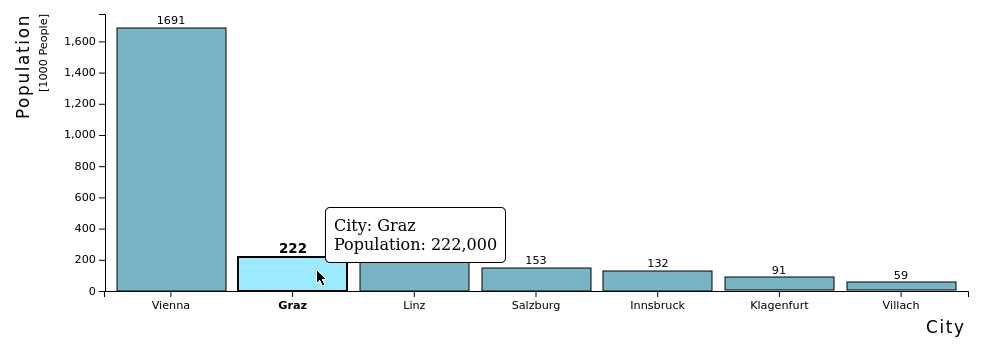
\includegraphics[keepaspectratio,width=\linewidth,height=\fullh]
{images/tooltip.png}
\caption[Tooltip Example]{%
A Bar Chart with an active Tooltip displaying
additional information for the data record associated with an
individual bar. Since a Tooltip is only visible during
interaction with a particular element, it may sometimes overlap
and cover other important parts of a Chart.
\imgcredit{Image created by the author of this thesis.}
}
\label{fig:Tooltip}
\end{figure}


The Tooltip package is located in the
\code{src/lib/tooltip/} directory of the RespVis library and contains
the implementation of Tooltips and utility functions to simplify the
configuration of Tooltips in Series modules. Tooltips are merely HTML
\elname{<div>} elements styled via CSS and can be initialized with the
\code{tooltip} function. Their visibility, position, and content is
controlled via the \code{tooltipShow}, \code{tooltipHide},
\code{tooltipPosition}, and \code{tooltipContent} functions in the
\code{tooltip.ts} file of the Tooltip package. Since RespVis
supports multiple simultaneous Tooltips, all of these functions have
to be passed the Tooltip element they should affect. Alternatively,
passing a \code{null} value operates on a default Tooltip element that
gets attached to the active documents \elname{<body>} element.
Tooltips are shown and hidden via the \code{tooltipShow} and
\code{tooltipHide} functions, which respectively add or remove the
\code{show} class to the Tooltip element. The actual showing and
hiding is done in CSS by setting the CSS \cssname{opacity} property of
the element depending on whether or not the \code{show} class is set.
Positions of Tooltips are configured via the \code{tooltipPosition}
function. This function calculates positions through an anchor
position in viewport coordinates and a directional offset from that
anchor. Specifying the anchor position is necessary, but the
directional offset can be omitted to have a sensible one chosen by the
\code{tooltipPosition} function, so that the Tooltip is always placed
inside the visible area of the browser. The actual positioning is
again done in CSS by setting a combination of the CSS \cssname{left},
\cssname{right}, \cssname{bottom}, and \cssname{top} properties
depending on the offset direction of the Tooltip. A Tooltip's content
can be set with the \code{tooltipContent} function, which sets the
Tooltip's inner HTML to the HTML string passed to the function.


Apart from Tooltips, the Tooltip package also contains
utility functions to simplify the setup and handling of Tooltips in
different Series modules such as the Bar or Point Series modules.
Interfaces describing the data objects of Series can inherit from the
\code{SeriesConfigTooltips} interface to add additional properties for
the configuration of Tooltips to these data objects. Among these
properties is a property to enable the Tooltips of the Series and
properties to specify the contents and positions of individual
Tooltips based on their associated context-element and the current
cursor position. In addition to the \code{SeriesConfigTooltips}
interface, the \code{seriesConfigTooltipsHandleEvents} function is
provided to automatically set \code{mouseover}, \code{mousemove}, and
\code{mouseout} event listeners on Series to automatically update the
visibility, content, and position of Tooltips based on the
\code{SeriesConfigTooltips} properties stored in the Series' data
object. The usage of these utilities is optional, and Series modules
are free to provide their own properties for the configuration of
Tooltips and their handling. However, for consistency reasons, the way
of configuring Tooltips should not differ too much between different
types of Series, and therefore it is recommended to use the utilities
provided here unless there is a good reason not to.

% KA TODO  There are no mouse events on touch, how solve?





\section{Bar Package}

A bar chart is used to compare the values of a quantitative variable
(values) uniquely associated with the distinct values of a qualitative
variable (categories), using rectangles whose lengths are
proportional to the values. Examples of datasets suitable for plotting
with a bar chart would be countries with their populations, people
with their ages, and web browsers with their market shares. Bar charts
have been in use for many centuries, with one of the earliest
documented occurrences being \textcite{CommercialAndPoliticalAtlas},
and are among the most frequently encountered types of visualizations
in the modern web.

The bars of a bar chart can be either horizontally or vertically
oriented. In horizontal bar charts, sometimes also called row charts,
categories are spread in equal intervals across the y-axis to define
the positions and heights of bars, and the associated values of
categories are mapped on the x-axis to determine their widths.
Conversely, in vertical bar charts, sometimes also called column
charts, categories are spread in equal intervals across the x-axis to
determine the positions and widths of bars, and the values of
categories are mapped on the y-axis to determine their heights.
Horizontal bar charts are better suited for display in narrow contexts
than vertical bar charts, because category labels can be positioned
more easily without having to rotate them and because these charts can
be vertically extended by having visualization consumers scroll
vertically, which is strongly preferable to scrolling horizontally.


The Bar package is located in the \code{src/lib/bars/} directory of
the RespVis library and contains modules to create single-series bar
charts, grouped multi-series bar charts, and stacked multi-series bar
charts that can be used in different situations. For every type of bar
chart, the Bar package provides a respective Series module to render
only the actual bars, a Chart module to render a full Chart including
a Bar Series, Axes, and a possible Legend, and a Chart Window module
to render a full Bar Chart embedded into a Layouter with additional
tools provided via a Toolbar. Higher-level modules are more convenient
to use, but they also impose more assumptions, and therefore
restrictions, on lower-level components contained within them. The
implementations of the different types of Bar Charts and when to best
use which type is described in the following sections.





\subsection{Single-Series Bar Modules}

Single-series bar charts are what most people think of when thinking
of bar charts. They consist of only a single series of bars and can
therefore only visualize differences between categories associated
with a single quantitative value at a time. The categories of a
single-series bar chart are mapped to spatial dimensions via a band
scale which partitions available space into equal intervals (bands)
with configurable padding between them. Thus, the width of bars is
calculated via the total number of categories, the range they are
spread on, and the padding between them. The mapping of quantitative
values to spatial dimensions in a single-series bar chart is performed
using a continuous scale, which maps quantitative values stored in a
dataset into a range of values between two extremes via a continuous
interpolation function. In most cases, linear interpolation via a
linear scale is used to map quantitative values, but visualization
authors can choose other forms of interpolation, such as logarithmic
interpolation via a logarithmic scale.

In RespVis, the Bar Series module renders collections of
\elname{<rect>} elements representing the bars in a Bar Chart's draw
area, and they are the lowest-level components required for rendering
Bar Charts. Their implementation is located in the
\code{series-bar.ts} file of the Bar package and contains the
\code{SeriesBar} interface describing data objects to configure Bar
Series, the \code{seriesBarData} function to create these data objects
from partial data objects, and the \code{seriesBarRender} function to
render Bar Series. The \code{SeriesBar} interface inherits Tooltip
configuration properties from the \code{SeriesConfigTooltips}
interface described in Section~\ref{sec:TooltipPackage} and adds
additional properties to configure the used categories and values, the
scales to map them to spatial dimensions, whether or not bars should
be oriented vertically or horizontally, and properties to configure
their colors and keys. After the desired \code{SeriesBar} data objects
have been created and bound to \elname{<svg>} or \elname{<g>}
elements, the \code{seriesBarRender} function can be used to render
Bar Series on these elements. During rendering, the bound
\code{SeriesBar} data object is transformed into an array of
\code{Bar} data objects, and a data join with these data objects is
performed to render the individual bars. The output range of the
scales used to map categories and values to spatial dimensions is set
to the dimensions of the Bar Series element's bounding box that has
been previously calculated and stored in the \attrname{bounds}
attribute by the Layouter. With these scales, the dimensions of bars
are calculated, and enter, update, and exit transitions are utilized
to interpolate them towards these new dimensions, so that changes are
easier to track, which leads to an improved experience for
visualization consumers. As with all other Series, the \code{enter},
\code{update}, and \code{exit} events containing the respective data
join Selections are dispatched on the Series' root element and allow
the injection of custom behavior into the different phases of the
Series' data join.

Bar Charts are Cartesian Charts, as discussed in
Section~\ref{sec:Chart}, which display a Bar Series with optional
labels in their draw area and visualize the scales used to map
categories and values to spatial dimensions as Axes. Their
implementation can be found in the \code{chart-bar.ts} file of the Bar
package, which contains the \code{ChartBar} interface to describe data
objects used for the configuration of Bar Charts, the
\code{chartBarData} function to create a fully initialized
\code{ChartBar} data object from a partial input object, and the
\code{chartBarRender} function to render Bar Charts into
\elname{<svg>} or \elname{<g>} elements to which \code{ChartBar} data
objects have been bound. The \code{ChartBar} interface inherits all
properties of the \code{ChartCartesian} and \code{SeriesBar}
interfaces and adds additional properties for the configuration of bar
labels. It is not necessary to manually specify all the offered
properties of this interface, because the \code{chartBarData} function
initializes all of them with sensible defaults derived from the
properties callers are interested in and which have been specified in
the partial data object passed to this function. The
\code{chartBarRender} function simply initializes a Cartesian Chart
and renders a Bar Series and an optional series of labels to annotate
the bars of the Bar Series into the Cartesian Chart's draw area.
Furthermore, the scales used for rendering the Bar Series are
visualized as Left and Bottom Axes of the Cartesian Chart, and a
\code{mouseover} event listener to highlight bars and their
corresponding ticks on the category axis is attached to bars.

Bar Chart Windows wrap a Bar Chart into a Layouter, so its elements
can be laid out with CSS. They also add a Toolbar containing tools to
filter a Bar Chart's categories and download an SVG version of the
current chart. Their implementation can be found in the
\code{chart-window-bar.ts} file of the Bar package, which contains the
\code{ChartWindowBar} interface to describe data objects for the
configuration of Bar Chart Windows, the \code{chartWindowBarData}
function to create a fully initialized \code{ChartWindowBar} data
object from a partial input object containing only relevant
properties, and the \code{chartWindowBarRender} function to render a
Bar Chart Window into \elname{<div>} elements onto which a
\code{ChartWindowBar} data object has been bound. The
\code{ChartWindowBar} interface inherits all properties of the
\code{ChartBar} interface to configure the wrapped Bar Chart and adds
additional properties needed for the filtering of categories. Bar
Chart Windows are rendered with the \code{chartWindowBarRender}
function, which renders a Toolbar including a Nominal Filtering Tool
for categories and an SVG Download Tool, initializes the nested Bar
Chart with the filtered values, and renders it, according to the
render process required by the Layouter defined in
Section~\ref{sec:Layouter}.


\begin{samepage}
\lstinputlisting[%
  float=tp,
  aboveskip=\floatsep,
  belowskip=\floatsep,
  xleftmargin=0cm,              % no extra margins for floats
  xrightmargin=0cm,             % no extra margins for floats
  %
  basicstyle=\footnotesize\ttfamily,
  frame=shadowbox,
  numbers=left,
  label=list:BarChartWindow,
  caption={[Code of Bar Chart Window Example]%
The source code to create the Bar Chart Window shown in
Figure~\ref{fig:BarChartWindow}. This Bar Chart Window is configured
with the bound data object initialized with the
\code{chartWindowBarData} function and rendered with the
\code{chartWindowBarRender} function. Since no special responsive
behavior is desired in this example, the default resize and category
filter behavior is attached to the Chart Window via the
\code{chartWindowBarAutoResize} and
\code{chartWindowBarAutoFilterCategories} functions.
},
]{listings/bar-chart-window.js}
\end{samepage}


By default, Bar Chart Windows are not automatically updated when the
viewport size changes or if their categories are filtered. Instead, a
custom \code{resize} event listener is attached to the Chart Window's
element, in which the Chart Window is responsively reconfigured
according to the changed viewport size and subsequently rerendered via
the \code{chartWindowBarRender} function. Furthermore, Bar Chart
Windows dispatch custom \code{categoryfilter} events containing the
currently active categories whenever categories are activated or
deactivated via the Nominal Filtering Tool. These events can be used
to responsively reconfigure Bar Chart Windows according to the
currently active categories by adding a custom \code{categoryfilter}
event listener which updates the configuration of the Bar Chart Window
accordingly and rerenders it. If no special configuration is required
when the viewport size or the category filtering changes, then the
\code{chartWindowBarAutoResize} and
\code{chartWindowBarAutoFilterCategories} functions can be used to
attach \code{resize} and \code{categoryfilter} event listeners that
implement the default behavior. A simple example of how a scalable Bar
Chart Window with filterable categories can be created is shown in
Listing~\ref{list:BarChartWindow} and the resulting visualization is
shown in Figure~\ref{fig:BarChartWindow}.



\begin{figure}[tp]
\centering
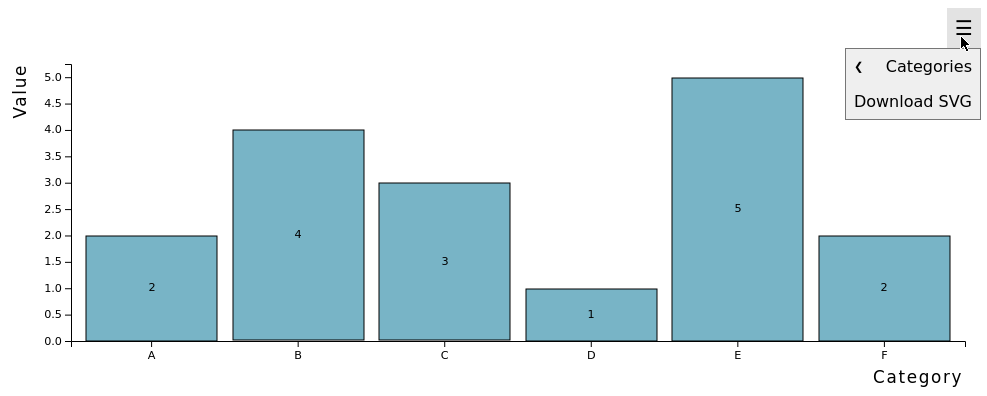
\includegraphics[keepaspectratio,width=\linewidth,height=\halfh]
{images/bar-chart-window.png}
\caption[Bar Chart Window Example]{%
The Bar Chart Window resulting from the code in
Listing~\ref{list:BarChartWindow}.
\imgcredit{Image created by the author of this thesis using RespVis.}
}
\label{fig:BarChartWindow}
\end{figure}






\subsection{Grouped Bar Modules}

Grouped bar charts, sometimes also called clustered or multi-series
bar charts, consist of multiple series of bars and are used to
visualize differences between categories, where each category is
associated with a number of quantitative variables. Every category
must be associated with the same number of quantitative variables,
effectively splitting categories into subcategories, and all values
assigned to these subcategories must be comparable with one another,
meaning they must have the same units and scales. As with
single-series bar charts, categories in grouped bar charts are also
mapped to spatial dimensions using band scales, but here, two
different band scales have to be applied. The category band scale
divides the available space along either the x or y-axis into equal
intervals based on the number of categories, whereas the subcategory
band scale further divides these intervals into even smaller intervals
based on the number of subcategories. Quantitative values are again
mapped to spatial dimensions via a single continuous scale.

In RespVis, the Bar package provides the Grouped Bar Series,
Grouped Bar Chart, and Grouped Bar Chart Window modules, which are
very similar to their Single-Series Bar Chart counterparts, to render
grouped bar charts in different levels of hierarchy. Grouped Bar
Series are the lowest-level components of these and render a
collection of \elname{<rect>} elements meant for display in the draw
area of a Grouped Bar Chart. The difference between a Grouped Bar
Series and a Single-Series Bar Series is that this one offers
additional properties needed for the configuration of subcategories
and that other properties specified as one-dimensional arrays in
Single-Series Bar Series are here required to hold two-dimensional
arrays so that their values can be assigned to the two-dimensionally
grouped bars. All bars belonging to the same subcategory have the same
style to simplify their comparison across all categories. 

Grouped Bar Charts are Cartesian Charts which contain a Grouped Bar
Series with optional labels in their draw area, Left and Bottom Axes
that visualize the scales used by this Grouped Bar Series, and a
Legend that visualizes the color-encoding of subcategories. These
Charts also attach event listeners to various elements to highlight
bars, labels, ticks on the category axis, and Legend items that
semantically belong together.

Grouped Bar Chart Windows contain a Grouped Bar Chart wrapped inside a
Layouter and render it following the render process defined in
Section~\ref{sec:Layouter} to allow positioning of their elements via
CSS. Furthermore, they decorate their nested Charts with Toolbars
containing tools to download them as SVG documents and filter their
categories and subcategories. Every time a visualization consumer
interacts with these Nominal Filtering Tools to change the
configuration of displayed categories and subcategories, the
\code{categoryfilter} and \code{subcategoryfilter} events are
dispatched, containing the newly active categories and subcategories
respectively. Visualization authors can either implement special
resize and filter behavior by attaching custom listeners to these
events, or can activate the default behavior via the
\code{chartWindowBarGroupedAutoResize},
\code{chartWindowBarGroupedAutoFilterCategories}, and
\code{chartWindowBarGroupedAutoFilterSubcategories} functions. Example
code to create a scalable Grouped Bar Chart Window whose categories
and subcategories can be filtered via the Toolbar is shown in
Listing~\ref{list:GroupedBarChartWindow} and the resulting
visualization is shown in Figure~\ref{fig:GroupedBarChartWindow}.



\begin{samepage}
\lstinputlisting[%
  float=tp,
  aboveskip=\floatsep,
  belowskip=\floatsep,
  xleftmargin=0cm,              % no extra margins for floats
  xrightmargin=0cm,             % no extra margins for floats
  %
  basicstyle=\footnotesize\ttfamily,
  frame=shadowbox,
  numbers=left,
  label=list:GroupedBarChartWindow,
  caption={[Code of Grouped Bar Chart Window Example]%
The source code to create the Grouped Bar Chart Window shown in
Figure~\ref{fig:GroupedBarChartWindow}. The Grouped Bar Chart Window
is configured via a bound data object, which is initialized with the
\code{chartWindowBarGroupedData} function and rendered with the
\code{chartWindowBarGroupedRender} function. Since no special
responsive behavior is desired in this example, the default resize,
category filter, and subcategory filter behavior is attached to the
Chart Window via the \code{chartWindowBarGroupedAutoResize},
\code{chartWindowBarGroupedAutoFilterCategories}, and
\code{chartWindowBarGroupedAutoFilterSubcategories} functions.
},
]{listings/grouped-bar-chart-window.js}
\end{samepage}


  
\begin{figure}[tp]
\centering
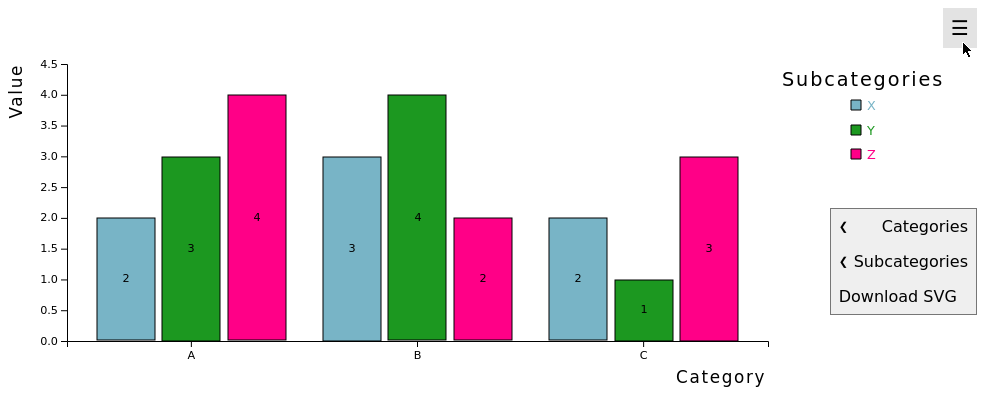
\includegraphics[keepaspectratio,width=\linewidth,height=\fullh]
{images/grouped-bar-chart-window.png}
\caption[Grouped Bar Chart Window Example]{%
The Grouped Bar Chart Window resulting from the source code in
Listing~\ref{list:GroupedBarChartWindow}. The Tool Menu popup has
been manually displaced to not cover the legend.
\imgcredit{Image created by the author of this thesis using RespVis.}
}
\label{fig:GroupedBarChartWindow}
\end{figure}








\subsection{Stacked Bar Modules}

Stacked bar charts are multi-series bar charts, in which individual
series of bars are rendered as stacks rather than as clusters. Since
the bars of stacked bar charts do not share a common baseline, these
charts are not well-suited for comparing individual subcategories
across multiple categories but rather for approximating the
contributions of subcategories to the totals of their categories. A
bar's color is determined by its subcategory so that all bars that
have the same subcategory are colored equally. Percent stacked bar
charts are variants of stacked bar charts, in which the totals of all
categories are transformed to equal 100\% by treating the quantitative
values of subcategories as ratios of a whole. Due to this
transformation, all stacks of bars are of equal length, meaning the
information about their totals is lost, but the share subcategories
contribute to their categories is emphasized more strongly than in
ordinary stacked bar charts. Bar stacks are created by splitting the
category axis into equal intervals via a band scale into which bars
representing the different subcategories are stacked on top of one
another. The lengths of stacked bars are proportional to their
quantitative values and are calculated via a continuous scale which
maps these values into the range of the value axis.


The RespVis library provides a Series, a Chart, and a Chart Window
module to render stacked bar charts, all of which are highly similar
to their grouped bar chart counterparts. Bars in Stacked Bar Series
are grouped two-dimensionally (category/subcategory), and
configuration properties affecting individual bars are specified as
two-dimensional arrays. The main difference between Stacked Bar Series
and Grouped Bar Series lies in how the positions and extents of bars
are calculated. Stacked Bar Charts are, just like Grouped Bar Charts,
Cartesian Charts consisting of a Stacked Bar Series with optional
labels, two Axes, and a Legend. Furthermore, Stacked Bar Chart Windows
are also equivalent to Grouped Bar Chart Windows as they wrap a
Stacked Bar Chart into a Layouter, manage their render
process, and decorate it with a Toolbar containing two Nominal
Filtering Tools to filter categories and subcategories. Percent
Stacked Bar Charts can be rendered either by directly setting
percentual values that lead to all category totals summing up to 100\%
or by enabling the \code{valuesAsRatios} configuration property, which
causes quantitative values to be treated as ratios which are
transformed to percentual shares of their category totals during
rendering. Listing~\ref{list:StackedBarChartWindow} shows example code
to create a scalable Stacked Bar Chart Window whose categories and
subcategories can be filtered. The chart itself is shown in
Figure~\ref{fig:StackedBarChartWindow}.
 

\begin{samepage}
\lstinputlisting[%
  float=tp,
  aboveskip=\floatsep,
  belowskip=\floatsep,
  xleftmargin=0cm,              % no extra margins for floats
  xrightmargin=0cm,             % no extra margins for floats
  %
  basicstyle=\footnotesize\ttfamily,
  frame=shadowbox,
  numbers=left,
  label=list:StackedBarChartWindow,
  caption={[Code of Stacked Bar Chart Window Example]%
The source code to create the Stacked Bar Chart Window shown in
Figure~\ref{fig:StackedBarChartWindow1}. The Stacked Bar Chart Window
is configured with the bound data object initialized via the
\code{chartWindowBarStackedData} function and rendered with the
\code{chartWindowBarStackedRender} function. Since no special
responsive behavior is desired in this example, the default resize,
category filter, and subcategory filter behavior is attached to the
Chart Window via the \code{chartWindowBarStackedAutoResize},
\code{chartWindowBarStackedAutoFilterCategories}, and
\code{chartWindowBarStackedAutoFilterSubcategories} functions.
Setting the \code{valuesAsRatios} variable to \code{true}
would result in the Percent Stacked Bar Chart shown in
Figure~\ref{fig:StackedBarChartWindow2}.
},
]{listings/stacked-bar-chart-window.js}
\end{samepage}





\begin{figure}[tp]
\centering
\subfloat[Stacked Bar Chart]{%
\hspace{1cm}
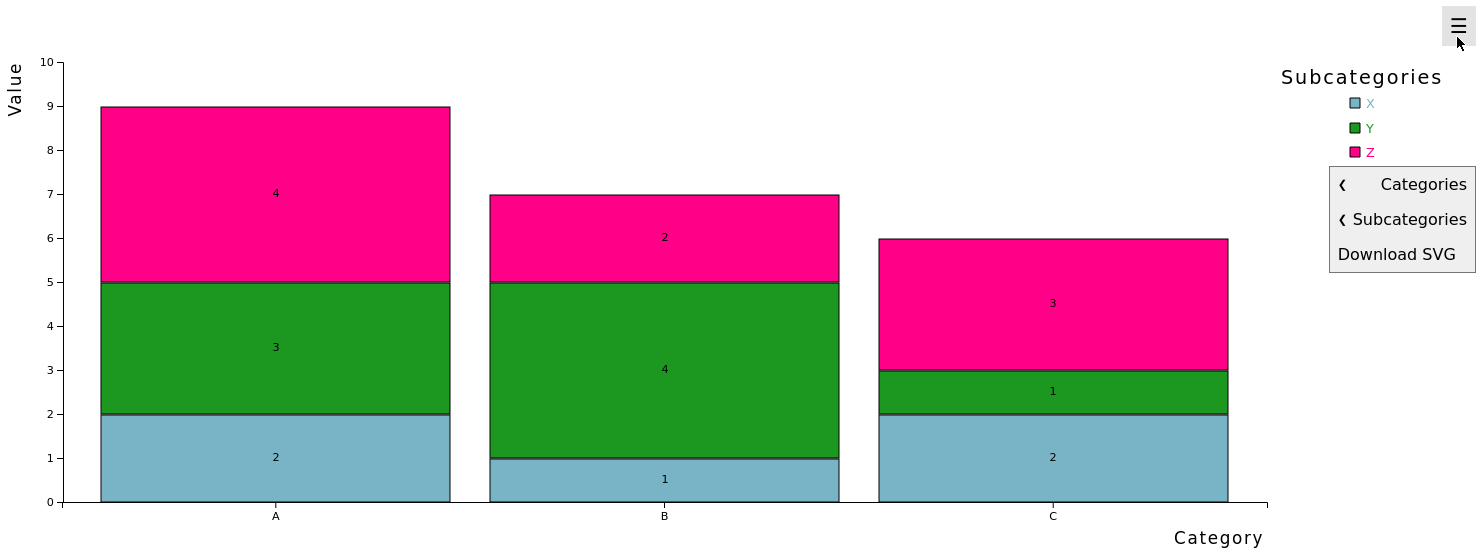
\includegraphics[keepaspectratio,width=\linewidth,height=\halfh]
{images/stacked-bar-chart-window.png}
\hspace{1cm}
\label{fig:StackedBarChartWindow1}
}
\hspace{1cm}
\subfloat[Percent Stacked Bar Chart]{%
\hspace{1cm}
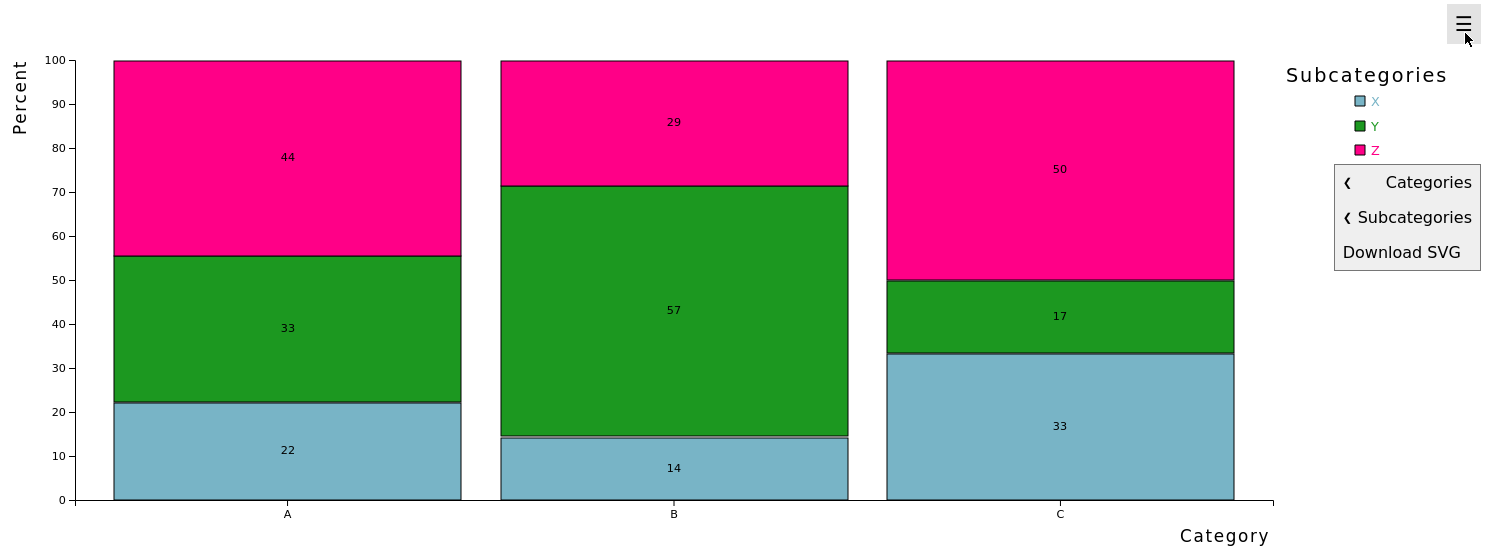
\includegraphics[keepaspectratio,width=\linewidth,height=\halfh]
{images/percent-stacked-bar-chart-window.png}
\hspace{1cm}
\label{fig:StackedBarChartWindow2}
}
\caption[Stacked Bar Chart Window Example]{%
The Stacked Bar Chart and Percent Stacked Bar Chart rendered by the source
code in Listing~\ref{list:StackedBarChartWindow}. The Tool Menu popup has
been manually displaced to not cover the legend.
\subref{fig:StackedBarChartWindow1} An ordinary Stacked Bar Chart to
compare category totals and subcategory contributions to these totals.
\subref{fig:StackedBarChartWindow2} A Percent Stacked Bar Chart to
better compare subcategory contributions to category totals.
\imgcredit{Image created by the author of this thesis using RespVis.}
}
\label{fig:StackedBarChartWindow}
\end{figure}
  




\section{Line Package}

Line charts show trends in data by plotting individual data records as
regularly-spaced markers connected by lines. The variables used to
position markers can be of any type as long as they can be spatially
encoded via scales. Usually, continuous scales are used to map
abstract variables to marker positions, but depending on the
variable's data types, any suitable type of scale that maps into the
respective axis' range can be used. Single-series line charts
visualize two-dimensional data via a single line, and multi-series
line charts visualize multi-dimensional data via multiple lines. In
multi-series line charts, each line represents a different variable
and is usually given a unique color. This color encoding is frequently
visualized via a legend.

The Line package is located in the \code{src/lib/line/} directory of
the RespVis library and contains modules to render Line Series, Line
Charts, and Line Chart Windows. A Line Series renders a collection of
\elname{<path>} elements representing polylines, whose individual
points are calculated by mapping arrays of x and y values into the
bounding box of the Series' root element via x and y scales. Line
Series support rendering multiple polylines by specifying multiple
arrays of y values which can all be mapped via the same scale. The
colors of individual polylines are specified via style classes.
Individual \elname{<path>} elements are rendered via a data join using
an array of data objects created by transforming the bound Series data
object. As with other Series, the data join can be customized via
custom \code{enter}, \code{update}, and \code{exit} event listeners.

Line Charts are Cartesian Charts which contain a Line Series, multiple
optional Point Series for the markers of individual lines, and
optional labels for these markers. Additionally, if a Line Chart
renders multiple lines and color-encodes them, a Legend is rendered by
the Line Chart. Marker labels and tooltips can be configured via the
Chart's data object. Furthermore, Line Charts attach mouse event
listeners to lines, markers, and legend items to highlight related
elements when hovering over one of them.


\begin{samepage}
\lstinputlisting[%
  float=tp,
  aboveskip=\floatsep,
  belowskip=\floatsep,
  xleftmargin=0cm,              % no extra margins for floats
  xrightmargin=0cm,             % no extra margins for floats
  %
  basicstyle=\footnotesize\ttfamily,
  frame=shadowbox,
  numbers=left,
  label=list:LineChartWindow,
  caption={[Code of Line Chart Window Example]%
The source code to create the Line Chart Window shown in
Figure~\ref{fig:LineChartWindow}. The Line Chart Window is
configured with a bound data object initialized with the
\code{chartWindowLineData} function and rendered with the
\code{chartWindowLineRender} function. Since no special responsive
behavior is desired in this example, the default resize behavior is
attached to the Chart Window via the \code{chartWindowLineAutoResize}
function.
},
]{listings/line-chart-window.js}
\end{samepage}



Line Chart Windows wrap a Line Chart into a Layouter, handle their
render process so that their elements can be laid out with CSS, and
decorate them with a Toolbar. By default, the Toolbars of Line Chart
Windows only contain an SVG Download Tool, because only a limited
number of Tools have been developed so far, and they are not
necessarily applicable to Line Charts. Depending on the type of data
visualized by a Line Chart, a Nominal Filtering Tool could be added to
the Toolbar. Once additional tools for different types of data, like a
tool to filter quantitative values, have been developed, they could
also be added to a Line Chart's Toolbar. Example source code to create
the scalable Line Chart Window shown in
Figure~\ref{fig:LineChartWindow} can be found in
Listing~\ref{list:LineChartWindow}.



\begin{figure}[tp]
\centering
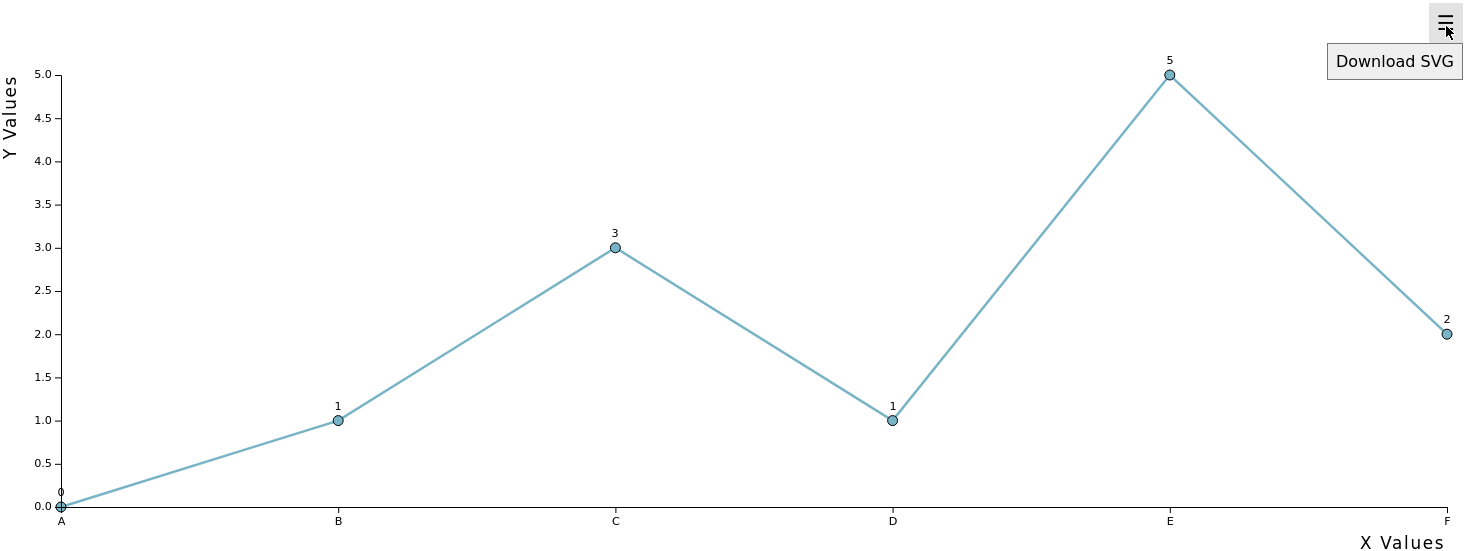
\includegraphics[keepaspectratio,width=\linewidth,height=\halfh]
{images/line-chart-window.png}
\caption[Line Chart Window Example]{%
The Line Chart Window resulting from the source code in
Listing~\ref{list:LineChartWindow}.
\imgcredit{Image created by the author of this thesis using RespVis.}
}
\label{fig:LineChartWindow}
\end{figure}





\section{Point Package}

Point charts, also commonly known as scatter charts or scatter plots,
show the relationship between two variables by plotting them as points
in a Cartesian coordinate system. Each of the two variables determines
a point's position on one of the coordinate system's two axes, and
typically, these variables contain quantitative data. However, the
data type of the variables used to position points is not relevant, as
long as their values can be mapped to spatial dimensions via scales.
Point charts are particularly suitable for discovering potential
correlations and patterns between variables. They can also visualize
more than two variables simultaneously by encoding additional
variables via the colors, sizes, and shapes of the plotted points.
Point charts which encode an additional variable as the sizes of
points are called bubble charts.


The Point package is located in the \code{src/lib/point/}
directory of the RespVis library and contains the Point Series, Point
Chart, and Point Chart Window modules. Point Series render a
collection of \elname{<circle>} elements, whose center positions are
calculated by mapping arrays of x and y values into the bounding boxes
of the Series' root elements via x and y scales. The colors of points
are specified as style classes, and their radiuses can be configured,
meaning that it is also possible to create bubble charts with these
modules. As with other Series, individual elements of Point Series are
rendered via a data join using an array of data objects created
through transforming the bound Series data object, and this data join
can be customized by providing custom \code{enter}, \code{update}, and
\code{exit} event listeners. Point Charts are Cartesian Charts which
contain Point Series in their draw areas and two Axes visualizing the
scales used to render the Point Series.




\begin{samepage}
\lstinputlisting[%
  float=tp,
  aboveskip=\floatsep,
  belowskip=\floatsep,
  xleftmargin=0cm,              % no extra margins for floats
  xrightmargin=0cm,             % no extra margins for floats
  %
  basicstyle=\footnotesize\ttfamily,
  frame=shadowbox,
  numbers=left,
  label=list:PointChartWindow,
  caption={[Code of Point Chart Window Example]%
The source code to create the Point Chart Window shown in
Figure~\ref{fig:PointChartWindow}. The Point Chart Window is
configured with a bound data object initialized with the
\code{chartWindowPointData} function and rendered with the
\code{chartWindowPointRender} function. Since no special responsive
behavior is desired in this example, the default resize behavior is
attached to the Chart Window via the \code{chartWindowPointAutoResize}
function.
},
]{listings/point-chart-window.js}
\end{samepage}


Point Chart Windows wrap a Point Chart into a Layouter,
handle the nested Chart's render process so that their elements can be
laid out with CSS, and decorate them with a Toolbar. Currently, the
Toolbars of Point Chart Windows only contain SVG Download Tools,
because only a limited number of Tools, not suited for application on
Point Charts, have been developed so far. Further Tools which can also
be applied to Point Charts, such as Zoom and Quantitative Filter
Tools, are planned for development, and once these are available, they
will be added to the default Tools attached to the Toolbars of Point
Chart Windows. Example source code to create a scalable Point Chart
Window can be found in Listing~\ref{list:PointChartWindow}, and the
resulting visualization is shown in Figure~\ref{fig:PointChartWindow}.



\begin{figure}[tp]
\centering
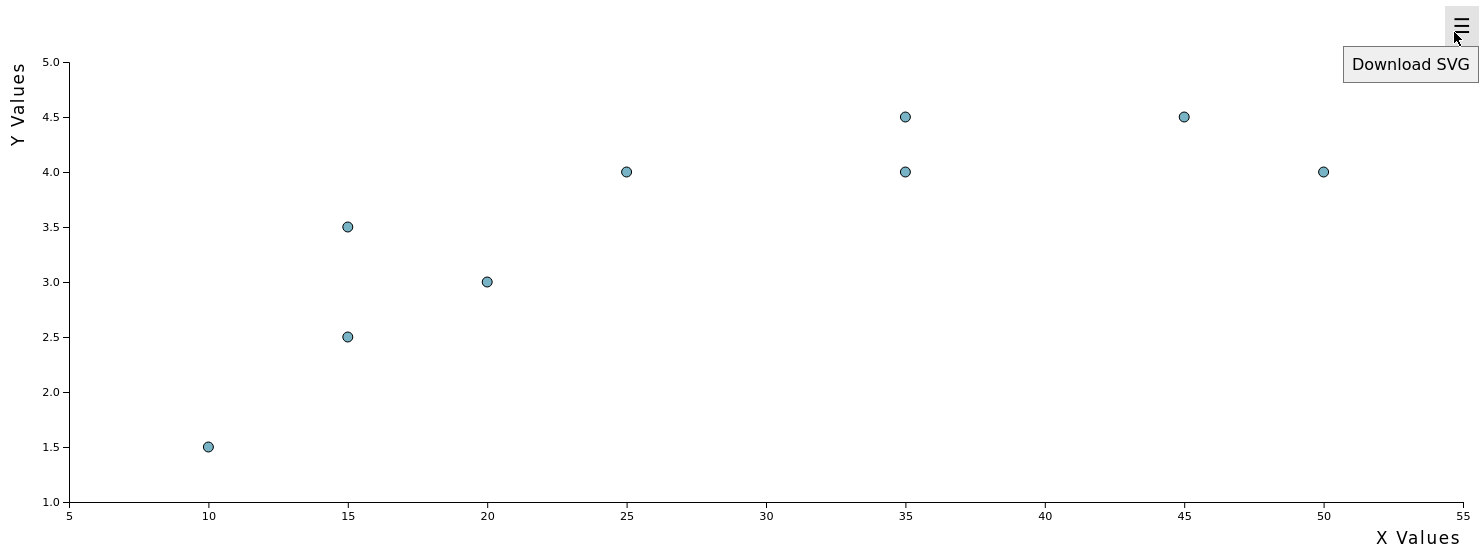
\includegraphics[keepaspectratio,width=\linewidth,height=\halfh]
{images/point-chart-window.png}
\caption[Point Chart Window Example]{%
The Point Chart Window resulting from the source code in
Listing~\ref{list:PointChartWindow}.
\imgcredit{Image created by the author of this thesis using RespVis.}
}
\label{fig:PointChartWindow}
\end{figure}
  
